\chapter{Wymagania funkcjonalne}
\label{chap3}
Poniższy rozdział opisuje funkcjonalności realizowanego systemu. Prezentuje wszystkie stawiane mu wymagania oraz założenia poczynione w trakcie ich analizy. Określa też profil jego odbiorcy oraz wyodrębnia aktorów tworzonej aplikacji.

%WYLECIALOPoniższy rozdział opisuje proces projektowania aplikacji. Przede wszystkim określa profil odbiorcy sytemu. Prezentuje też wszystkie wymagania oraz założenia poczynione w trakcie ich analizy.

\section[Profil odbiorcy systemu][Profil odbiorcy systemu]{Profil odbiorcy systemu}
Potrzeba stworzenia systemu do obsługi umów cywilno-prawnych powstała na Politechnice Warszawskiej, a dokładniej w Ośrodku Kształcenia na Odległość. Początkowa miała ona obsługiwać jedynie umowy zlecenia, jednak zdecydowano się ją rozszerzyć również na umowy o dzieło (stąd ogólna nazwa umowy cywilno-prawne). Podczas procesu projektowania starano się, aby model był nie tylko dostosowany do specyfiki uczelni, ale też jak najbardziej ogólny. Dzięki temu potencjalnym odbiorcą aplikacji mogą być nie tylko uczelnie, ale i inne instytucje o podobnej strukturze organizacyjnej.

\section[Opis funkcjonalności][Opis funkcjonalności]{Opis funkcjonalności}

\subsection[Pracownicy][Pracownicy]{Pracownicy}
\label{pracownicy}
Aplikacja powinna umożliwiać przechowywanie danych o osobach zatrudnianych na umowach cywilno-prawnych, zwanych dalej potocznie pracownikami (nie są to pracownicy w rozumieniu kodeksu pracy). Podstawowymi operacjami jakie można wykonać na pracowniku jest jego dodanie, modyfikacja oraz usunięcie (ale tylko w przypadku, gdy nie ma on podpisanej żadnej umowy). Dodatkowymi funkcjonalnościami są wyszukiwanie pracownika za pomocą imienia i nazwiska oraz możliwość wyświetlenia listy wszystkich pracowników.

Aplikacja będzie gromadzić wszystkie informacje niezbędne do jednoznacznej identyfikacji pracownika oraz dane umieszczane na umowach czy też potrzebne w celach podatkowych: nazwisko, imiona (z wyróżnieniem pierwszego imienia), adresy (przy czym należy zwrócić uwagę, że adres zamieszkania wykorzystywany w celach podatkowych może różnić się od adresu zameldowania umieszczanego na umowie oraz że pracownik może posiadać jeszcze adres korespondencyjny), datę i miejsce urodzenia, płeć, obywatelstwo (aplikacja powinna udostępniać wybór z listy możliwych państw), numery PESEL oraz NIP, numer dowodu osobistego lub paszportu oraz numer konta. Dodatkowo system powinien przechowywać informację o urzędzie skarbowym (jego nazwę i adres) właściwym dla pracownika. Dane urzędu skarbowego powinny być przechowywane niezależnie od danych pracownika tak aby np. w przypadku zmiany adresu jednego z urzędów nie występowała konieczność ręcznej aktualizacji wszystkich odpowiadających mu pracowników a jedynie pojedyncza modyfikacja danych urzędu skarbowego. Podczas wprowadzania bądź modyfikacji danych pracownika użytkownik powinien mieć możliwość wyboru urzędu skarbowego z ich ogólnopolskiej listy. 

Istotnym elementem danych pracownika jest informacja, jakie składki ubezpieczeń będzie musiał odprowadzać od potencjalnie podpisanych umów. Aplikacja powinna przechowywać informacje o jego statusie z punktu widzenia umów cywilno prawnych (opisanym w \ref{przykladyOsob}). Powinna też wspomagać użytkownika w trakcie wyboru statusu - wyświetlać ich szczegółowe opisy oraz powiązane z nimi składki ubezpieczeń. Te informacje powinny być również zawarte w raportach prezentujących dane pracownika. Lista dostępnych statusów jest zdefiniowana w momencie instalacji, nie ma możliwości jej edycji za pomocą aplikacji.

\subsection[Struktura organizacyjna][Struktura organizacyjna]{Struktura organizacyjna}
Struktura organizacyjna uczelni podobnie jak struktura organizacyjna wielu innych instytucji ma formę drzewa. Dla prawie każdej jednostki organizacyjnej można wskazać jednostkę nadrzędną (wyjątkiem jest jednostka będąca korzeniem drzewa, z reguły jest to sama organizacja, np. konkretna uczelnia). Ponadto jednostki na poszczególnych poziomach drzewa posiadają swoje typy. W przypadku Politechniki Warszawskiej są to m. in. uczelnia, wydział, instytut czy zakład. Nie jest jednak wymogiem, aby na jednym poziomie drzewa znajdowały się jednostki tylko jednego typu. Na przykład jednostkami podległymi wydziałowi mogą być nie tylko instytuty, ale też dziekanat, czy administracja gmachu. Nie ma też wymogu, aby jednostką nadrzędną danej jednostki organizacyjnej była jednostka typu, który jest typem bezpośrednio nadrzędnym w stosunku do jej typu. Na przykład nie wszystkie zakłady muszą podlegać instytutom, niektóre z nich mogą podlegać bezpośrednio wydziałom. 

Aplikacja powinna udostępniać zestaw typów jednostek oraz definiować ich wzajemną hierarchię. Dane te powinny być zdefiniowane w momencie instalacji i nie powinno być możliwości ich zmiany z poziomu aplikacji. Program powinien umożliwiać dodawanie nowych jednostek organizacyjnych (nadawanie im nazwy), definiowanie ich typów oraz umieszczanie ich w strukturze organizacji (poprzez nadawanie jednostek nadrzędnych). Powinien również umożliwiać ich edycję oraz usuwanie (pod warunkiem, że nie spowoduje to osierocenia innej jednostki organizacyjnej oraz w systemie nie ma zdefiniowanych zadań wykonywanych dla tej jednostki (patrz \ref{zadania})). Aplikacja powinna pilnować struktury drzewa oraz zgodności typów jednostek. Powinna też umożliwiać wyszukiwanie jednostki za pomocą jej nazwy, oraz wyświetlanie wszystkich jednostek obecnych w systemie.

Atrybutami jednostki oprócz wspominanych wcześniej nazwy, typu i miejsca w strukturze organizacji są jej adres oraz reprezentant, którego zadaniem jest podpisywanie umów w imieniu jednostki. Atrybutami reprezentanta są jego imię i nazwisko, jednak ze względu pisemną formę umowy należy przechowywać również ich formę biernika. Jeden reprezentant może być przypisany do kliku jednostek. Podczas wprowadzania bądź modyfikacji jednostki użytkownik powinien mieć możliwość wyboru reprezentanta z listy już wcześniej wprowadzonych lub dodania nowego w przypadku jego braku na liście.

%W trakcie analizy podjęto decyzję, że pracownicy nie będą w żaden sposób połączeni z jedną konkretną jednostką (nawet jeśli są w niej na stałe zatrudnieni).

\subsection[Zadania][Zadania]{Zadania}
\label{zadania}
W ramach jednostek organizacyjnych wykonywane są zadania. Na wykonywanie poszczególnych zadań, bądź ich części, zatrudnia się pracowników na umowy cywilno-prawne. Podstawowym atrybutem zadania jest jego nazwa. Zadanie może też posiadać swój opis, budżet, datę rozpoczęcia oraz datę zakończenia. O ile opis pełni charakter jedynie informacyjny, to w przypadku pozostałych atrybutów aplikacja powinna sprawdzać czy umowy podpisywane na wykonanie tego zadanie mieszczą się w zdefiniowanych ramach czasowych (data rozpoczęcia i data zakończenia) oraz czy sumaryczna wartość umów nie przekracza budżetu zdefiniowanego dla danego zadania. Dodatkowo istnieje możliwość oznaczenia zadania jako rozliczone skutkująca tym, że nie będzie można podpisywać już żadnych umów na wykonywanie tego zadania. 

Istnieje także możliwość podziału zadań na mniejsze grupy w ramach poszczególnych jednostek organizacyjnych. Służy do tego atrybut typ zadania (definiowany w ramach jednostki).
%Podczas analizy ustalono, że powinna istnieć możliwość podziału zadań na mniejsze grupy w ramach jednostki organizacyjnej. Wprowadzono więc kolejny atrybut zadania jakim jest jego typ (definiowany w ramach jednostki). 

Użytkownik powinien posiadać możliwość dodawania i edycji zarówno zadań jak i ich typów. Usuwanie typów zadań możliwe jest tylko wtedy, gdy nie ma żadnego zadania danego typu. Analogicznie usunąć zadanie można tylko wtedy gdy w systemie nie ma żadnych powiązanym z nim umów. Dodatkowo system powinien umożliwiać wyszukiwanie zadań po nazwie oraz ich typie, oraz wyświetlanie wszystkich zadań powiązanych z daną jednostką organizacyjną oraz jednostkami jej podległymi. Analogicznie użytkownik powinien mieć możliwość wyszukiwania typów zadań po ich nazwach oraz możliwość wyświetlania wszystkich typów zadań właściwych dla danej jednostki.

\subsection[Umowy][Umowy]{Umowy}
Najważniejszym obiektem występującym w systemie jest umowa. Podstawowymi atrybutami umowy są jej strony, a więc jednostka organizacyjna oraz pracownik. Umowa zawiera też: daty zawarcia, rozpoczęcia i zakończenia (przy czym system pilnuje aby data zawarcia była wcześniejsza lub taka sama jak data rozpoczęcia oraz aby data zakończenia była późniejsza niż data rozpoczęcia). Zawiera również przedmiot umowy (nazwę dzieła lub zlecenia), wynagrodzenie jakie należy się za jego wykonanie oraz informację czy umowa będzie wykonywana w siedzibie zlecającego. 

\subsubsection{Typ umowy}
Użytkownik ma możliwość wyboru typu umowy. Typ umowy definiuje tytuł umowy (umowa zlecenia czy o dzieło) oraz koszt uzyskania przychodu. W projektowanej wersji aplikacji dostępne będą standardowe stawki kosztu uzyskania przychodu wynoszące 20\% i 50\%. Typ umowy posiada również nazwę. Jest ona w ogólnym przypadku różna od tytułu umowy, np. dla typu o nazwie \textit{Umowa o dzieło autorskie} tytułem umowy będzie \textit{Umowa o dzieło}. Na podstawie typu oraz wynagrodzenia z tytułu umowy, a także na podstawie statusu, wieku oraz płci pracownika określane będzie, jakie składki będą musiały być odprowadzone od umowy. W przypadku składek dobrowolnych użytkownik pytany jest czy pracownik jest zainteresowany ich odprowadzaniem. Typy umowy są zdefiniowane w systemie w momencie instalacji. Analogicznie do innych elementów tego typu nie ma możliwości ich edycji za pomocą aplikacji.

\subsubsection{Płatność}
Użytkownik ma możliwość wyboru jednego ze zdefiniowanych sposobu płatności. Podstawowym sposobem płatności jest płatność jednorazowa po zakończeniu umowy. System umożliwia też wybór ratalnego sposobu płatności, gdzie okres między kolejnymi ratami może być zdefiniowany w dniach albo miesiącach. Użytkownik ma możliwość samodzielnego definiowana sposobów płatności podając ich nazwę oraz liczbę dni lub miesięcy, co jakie powinno być wypłacane wynagrodzenie. Ma też możliwość usuwania zdefiniowanych przez siebie wcześniej a nie używanych sposobów płatności. 

\subsubsection{Numer umowy}
Numery umów będą nadawane automatycznie przez aplikację. Sygnatura umowy powinna być unikalna w skali całego systemu. Przyjęto założenie, że częścią składową numeru umowy będzie data jej zawarcia (w formie numerycznej). Numer umowy będzie umieszczany w jej nagłówku.

\subsubsection{}
Użytkownik ma możliwość dodawania nowych umów, ich edycji oraz usuwania. System umożliwia ponadto wyświetlanie listy wszystkich umów dostępnych dla danego użytkownika oraz pozwala na ich wyszukiwanie na podstawie pracownika, jednostki oraz zadania.

\subsection[Rachunki][Rachunki]{Rachunki}
Jako postawę do wypłaty wynagrodzenia przyjęto rachunek. Rachunki występują zawsze w kontekście danej umowy. Są one ponadto numerowane (numeyr rachunków są kolejnymi liczbami naturalnymi). Atrybutami rachunku są ponadto kwota oraz data wystawienia.

Rachunki będą generowanie przez aplikację automatycznie na podstawie wybranego sposobu płatności. Użytkownik będzie miał jedynie możliwość ich wyświetlania. Usunięcie rachunków możliwe jest jedynie przez usunięcie powiązanej z nimi umowy, a ich modyfikacja może odbywać się poprzez zmianę parametrów umowy (wynagrodzenia i sposobu płatności).

\subsection[Wydruki][Wydruki]{Wydruki}
Użytkownik będzie miał możliwość wydruku zarówno umów jak i rachunków. Zrealizowane zostanie to poprzez udostępnienie ich w formacie pdf. Wydruki umów będą generowane wg wzorców różnych dla każdego typu umowy.

\section[Aktorzy][Aktorzy]{Aktorzy}
W aplikacji zostali wyróżnieni dwaj aktorzy:

\subsubsection{Administrator jednostki}
Powiązany z konkretną jednostką organizacyjną, ma możliwość wykonywania operacji na zadaniach, typach zadań oraz umowach w ramach swojej jednostki oraz wszystkich jednostek jej podlegających. Może mieć możliwość wykonywania operacji na pracownikach.
%TODO co z pracownikami

\subsubsection{Administrator systemu}
Ma możliwość wykonywania operacji na jednostkach organizacyjnych oraz zarządzania administratorami jednostek (ich dodawanie, usuwanie oraz przydzielanie uprawnień). Może definiować nowe sposoby płatności. Ma uprawnienia administratora jednostki dla wszystkich jednostek organizacyjnych obecnych w systemie.

\section[Przypadki użycia][Przypadki użycia]{Przypadki użycia}
Jednym z etapów modelowania aplikacji jest określenie przypadków użycia (ang. \textit{Use Case}). Przypadkami użycia nazywamy funkcjonalności systemu z punktu widzenia użytkownika. Przypadki użycia mogą się w sobie zawierać oraz się rozszerzać. Z punktu widzenia przejrzystości dokumentacji dobrą praktyką jest numerowanie przypadków użycia.

\subsection[Diagram przypadków użycia][Diagram przypadków użycia]{Diagram przypadków użycia}
Diagram przypadków użycia jest graficzną formą ich prezentacji. Zawiera on jedynie aktorów oraz funkcjonalności modelowane systemu. Nie dostarcza informacji o sposobie realizacji tych funkcjonalności. Wybrany diagram przypadków użycia zamieszczono na rysunku \ref{diagram-uc}.


\begin{figure}[tdh]
    \begin{center}
	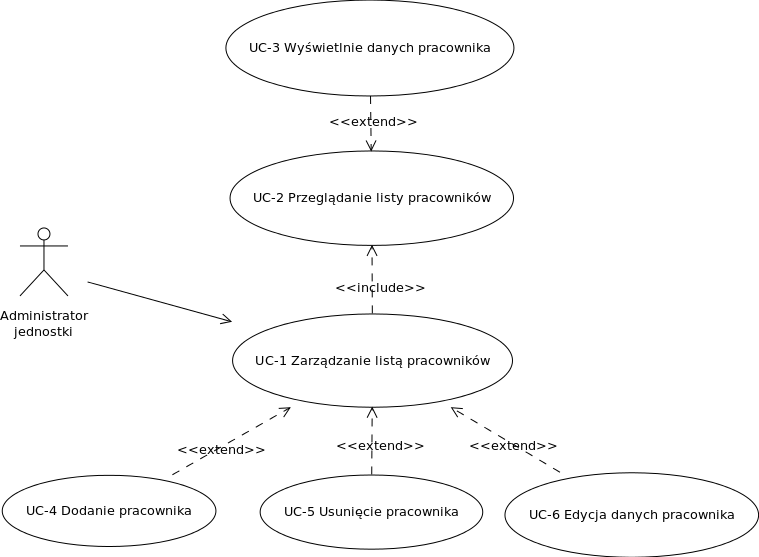
\includegraphics[scale=.6]{img/diagram-uc.png}
	\caption{Diagram przypadków użycia dla zarządzania listą pracowników}
	\label{diagram-uc}
    \end{center}
\end{figure}


\subsection[Scenariusze przypadków użycia][Scenariusze przypadków użycia]{Scenariusze przypadków użycia}
Więcej informacji o poszczególnych funkcjonalnościach systemu dostarczają scenariusze przypadków użycia. Opisują one w sposób słowny aktorów biorących udział w danych przypadku, warunki wstępne oraz końcowe. Opisują też szczegółowo interakcję pomiędzy użytkownikiem a systemem. Wyróżnić można dwie formy takiego opisu: opis w postaci ciągłego tekstu oraz listę kroków. Poniżej przedstawiony został wybrany scenariusz dla przypadku dodawania pracownika:

\paragraph{UC-4 Dodawanie pracownika}
rozszerza UC-1 zarządzanie listą pracowników.\\
\begin{tabular}{ll}
	\textbf{Aktorzy:} & Administrator jednostki \\
	
	\textbf{Warunek początkowy:} & Użytkownik zalogowany w systemie \\
	\textbf{Warunek końcowy:} & Nowy pracownik zapisany w systemie \\
	\multicolumn{2}{l}{\textbf{Scenariusz główny:}}\\
	\multicolumn{2}{l}{
	\begin{minipage}{\textwidth}\begin{enumerate}
		\item Użytkownik wybiera opcję "Dodaj nowego pracownika".
		\item System wyświetla formularz dodawania użytkownika.
		\item Użytkownik wypełnia formularz.
		\item Użytkownik potwierdza przesłanie formularza przyciskiem "Wprowadź".
		\item System sprawdza poprawność wprowadzonych danych.
		\item System zapisuje dane nowego pracownika
	\end{enumerate}\end{minipage}
	}
\end{tabular}
	
\section[Prototypowanie][Prototypowanie]{Prototypowanie}
Po zakończeniu etapu analizy możliwe jest stworzenie makiet realizowanego systemu. Makiety nie odzwierciedlają faktycznego wyglądu aplikacji, zawierają jednak wszystkie jej elementy w postaci uproszczonych kontrolek. Pozwalają na szersze spojrzenie na całość projektowanego systemu co niekiedy może prowadzić do wychwycenia błędów w jej modelu logicznym. Makiety są wreszcie cenną pomocą dla programistów mających mniejsze doświadczenie w pracy nad częścią kliencką aplikacji. Wybrane makiety zaprezentowane zostały w dodatku \ref{makiety}. Zostały one wykonane za pomocą programu Balsamiq Mockup.


